\documentclass[11pt,preprint]{elsarticle}

\usepackage{lmodern}
%%%% My spacing
\usepackage{setspace}
\setstretch{1.2}
\DeclareMathSizes{12}{14}{10}{10}

% Wrap around which gives all figures included the [H] command, or places it "here". This can be tedious to code in Rmarkdown.
\usepackage{float}
\let\origfigure\figure
\let\endorigfigure\endfigure
\renewenvironment{figure}[1][2] {
    \expandafter\origfigure\expandafter[H]
} {
    \endorigfigure
}

\let\origtable\table
\let\endorigtable\endtable
\renewenvironment{table}[1][2] {
    \expandafter\origtable\expandafter[H]
} {
    \endorigtable
}


\usepackage{ifxetex,ifluatex}
\usepackage{fixltx2e} % provides \textsubscript
\ifnum 0\ifxetex 1\fi\ifluatex 1\fi=0 % if pdftex
  \usepackage[T1]{fontenc}
  \usepackage[utf8]{inputenc}
\else % if luatex or xelatex
  \ifxetex
    \usepackage{mathspec}
    \usepackage{xltxtra,xunicode}
  \else
    \usepackage{fontspec}
  \fi
  \defaultfontfeatures{Mapping=tex-text,Scale=MatchLowercase}
  \newcommand{\euro}{€}
\fi

\usepackage{amssymb, amsmath, amsthm, amsfonts}

\def\bibsection{\section*{References}} %%% Make "References" appear before bibliography


\usepackage[numbers]{natbib}

\usepackage{longtable}
\usepackage[margin=2.3cm,bottom=2cm,top=2.5cm, includefoot]{geometry}
\usepackage{fancyhdr}
\usepackage[bottom, hang, flushmargin]{footmisc}
\usepackage{graphicx}
\numberwithin{equation}{section}
\numberwithin{figure}{section}
\numberwithin{table}{section}
\setlength{\parindent}{0cm}
\setlength{\parskip}{1.3ex plus 0.5ex minus 0.3ex}
\usepackage{textcomp}
\renewcommand{\headrulewidth}{0.2pt}
\renewcommand{\footrulewidth}{0.3pt}

\usepackage{array}
\newcolumntype{x}[1]{>{\centering\arraybackslash\hspace{0pt}}p{#1}}

%%%%  Remove the "preprint submitted to" part. Don't worry about this either, it just looks better without it:
\makeatletter
\def\ps@pprintTitle{%
  \let\@oddhead\@empty
  \let\@evenhead\@empty
  \let\@oddfoot\@empty
  \let\@evenfoot\@oddfoot
}
\makeatother

 \def\tightlist{} % This allows for subbullets!

\usepackage{hyperref}
\hypersetup{breaklinks=true,
            bookmarks=true,
            colorlinks=true,
            citecolor=blue,
            urlcolor=blue,
            linkcolor=blue,
            pdfborder={0 0 0}}


% The following packages allow huxtable to work:
\usepackage{siunitx}
\usepackage{multirow}
\usepackage{hhline}
\usepackage{calc}
\usepackage{tabularx}
\usepackage{booktabs}
\usepackage{caption}


\newenvironment{columns}[1][]{}{}

\newenvironment{column}[1]{\begin{minipage}{#1}\ignorespaces}{%
\end{minipage}
\ifhmode\unskip\fi
\aftergroup\useignorespacesandallpars}

\def\useignorespacesandallpars#1\ignorespaces\fi{%
#1\fi\ignorespacesandallpars}

\makeatletter
\def\ignorespacesandallpars{%
  \@ifnextchar\par
    {\expandafter\ignorespacesandallpars\@gobble}%
    {}%
}
\makeatother


% definitions for citeproc citations
\NewDocumentCommand\citeproctext{}{}
\NewDocumentCommand\citeproc{mm}{%
\href{\#cite.\detokenize{#1}}{#2}\nocite{#1}}

\makeatletter
% allow citations to break across lines
\let\@cite@ofmt\@firstofone
% avoid brackets around text for \cite:
\def\@biblabel#1{}
\def\@cite#1#2{{#1\if@tempswa , #2\fi}}
\makeatother
\newlength{\cslhangindent}
\setlength{\cslhangindent}{1.5em}
\newlength{\csllabelwidth}
\setlength{\csllabelwidth}{3em}
\newenvironment{CSLReferences}[2] % #1 hanging-indent, #2 entry-spacing
{\begin{list}{}{%
	\setlength{\itemindent}{0pt}
	\setlength{\leftmargin}{0pt}
	\setlength{\parsep}{0pt}
	% turn on hanging indent if param 1 is 1
	\ifodd #1
	\setlength{\leftmargin}{\cslhangindent}
	\setlength{\itemindent}{-1\cslhangindent}
	\fi
	% set entry spacing
	\setlength{\itemsep}{#2\baselineskip}}}
{\end{list}}

\usepackage{calc}
\newcommand{\CSLBlock}[1]{\hfill\break\parbox[t]{\linewidth}{\strut\ignorespaces#1\strut}}
\newcommand{\CSLLeftMargin}[1]{\parbox[t]{\csllabelwidth}{\strut#1\strut}}
\newcommand{\CSLRightInline}[1]{\parbox[t]{\linewidth - \csllabelwidth}{\strut#1\strut}}
\newcommand{\CSLIndent}[1]{\hspace{\cslhangindent}#1}


\urlstyle{same}  % don't use monospace font for urls
\setlength{\parindent}{0pt}
\setlength{\parskip}{6pt plus 2pt minus 1pt}
\setlength{\emergencystretch}{3em}  % prevent overfull lines
\setcounter{secnumdepth}{5}

%%% Use protect on footnotes to avoid problems with footnotes in titles
\let\rmarkdownfootnote\footnote%
\def\footnote{\protect\rmarkdownfootnote}
\IfFileExists{upquote.sty}{\usepackage{upquote}}{}

%%% Include extra packages specified by user
\usepackage{sectsty}
\sectionfont{\bfseries\large}
\subsectionfont{\bfseries\normalsize}

%%% Hard setting column skips for reports - this ensures greater consistency and control over the length settings in the document.
%% page layout
%% paragraphs
\setlength{\baselineskip}{12pt plus 0pt minus 0pt}
\setlength{\parskip}{12pt plus 0pt minus 0pt}
\setlength{\parindent}{0pt plus 0pt minus 0pt}
%% floats
\setlength{\floatsep}{12pt plus 0 pt minus 0pt}
\setlength{\textfloatsep}{20pt plus 0pt minus 0pt}
\setlength{\intextsep}{14pt plus 0pt minus 0pt}
\setlength{\dbltextfloatsep}{20pt plus 0pt minus 0pt}
\setlength{\dblfloatsep}{14pt plus 0pt minus 0pt}
%% maths
\setlength{\abovedisplayskip}{12pt plus 0pt minus 0pt}
\setlength{\belowdisplayskip}{12pt plus 0pt minus 0pt}
%% lists
\setlength{\topsep}{10pt plus 0pt minus 0pt}
\setlength{\partopsep}{3pt plus 0pt minus 0pt}
\setlength{\itemsep}{5pt plus 0pt minus 0pt}
\setlength{\labelsep}{8mm plus 0mm minus 0mm}
\setlength{\parsep}{\the\parskip}
\setlength{\listparindent}{\the\parindent}
%% verbatim
\setlength{\fboxsep}{5pt plus 0pt minus 0pt}



\begin{document}



\begin{frontmatter}  %

\title{Macroeconomics Assignment}

% Set to FALSE if wanting to remove title (for submission)




\author[Add1]{Liam Andrew Beattie}
\ead{22562435@sun.ac.za}





\address[Add1]{Macroeconomics 871, Stellenbosch University, South
Africa}


\begin{abstract}
\small{
Almost an abstract
}
\end{abstract}

\vspace{1cm}





\vspace{0.5cm}

\end{frontmatter}

\setcounter{footnote}{0}



%________________________
% Header and Footers
%%%%%%%%%%%%%%%%%%%%%%%%%%%%%%%%%
\pagestyle{fancy}
\chead{}
\rhead{}
\lfoot{}
\rfoot{\footnotesize Page \thepage}
\lhead{}
%\rfoot{\footnotesize Page \thepage } % "e.g. Page 2"
\cfoot{}

%\setlength\headheight{30pt}
%%%%%%%%%%%%%%%%%%%%%%%%%%%%%%%%%
%________________________

\headsep 35pt % So that header does not go over title




I have used an R package from Mati (\citeproc{ref-Mati2019}{2019}) and
should give credit. This allowed me to code everything in R while still
using Dynare.

\section{Model Specification}\label{model-specification}

Above could note be a heading on itself. Just a paragraph that it is a
core rbc foundations and what that means.

Note that capital letters denote nominal amounts and lowercase denote
real values.

Mainly adding capital to Sims
(\citeproc{ref-sims2024newkeynesian}{2024a}), while also introducing
adjustment costs from Sims (\citeproc{ref-sims2024rbc}{2024b}) .
Rotemberg prices was used while gleeming insights from European Central
Bank (\citeproc{ref-ecbwp770}{2022}) .

\subsection{Households}\label{households}

\begin{equation}
C_t \;=\; P_t \, c_t,
\qquad
I_t \;=\; P_t \, i_t
\label{nominal_definitions}
\end{equation}

\begin{equation}
\max_{\{C_t,\,h_t,\,M_t,\,B_t,\,K_t,\,I_t\}}
\mathbb{E}_0 \sum_{t=1}^{\infty} \beta^{t-1}
\left[
\frac{\Bigl(\frac{C_t}{P_t} - \eta\,\frac{C_{t-1}}{P_{t-1}}\Bigr)^{1-\theta}}{1-\theta}
\;-\;\chi\,\frac{h_t^{1+\gamma}}{1+\gamma}
\;+\;\psi\,\ln\!\Bigl(\frac{M_t}{P_t}\Bigr)
\right]
\label{lifetime_utility_nominal}
\end{equation}

\begin{equation}
C_t \;+\; I_t \;+\; B_t \;+\; M_t
\;\le\;
R^B_{\,t-1}\,B_{t-1}
\;+\; M_{t-1}
\;+\; W_t\,h_t
\;+\; R^k_t\,K_{t-1}
\;+\; \Pi_t
\;-\; P_t\,\tau_t
\label{flow_constraint_nominal}
\end{equation}

\begin{equation}
K_t
\;=\;
(1 - \delta)\,K_{t-1}
\;+\; I_t
\;-\;\frac{\phi}{2}
\left(\frac{I_t}{K_{t-1}} - \delta\right)^{2}
\,K_{t-1}
\label{capital_accumulation_nominal}
\end{equation}

From which we can derive the following equations, found in full form in
Appendix \ref{household_FOC}

\begin{equation}\label{consEuler}
  (c_t - \eta\,c_{t-1})^{-\theta}
  \;=\;
  \beta\,\mathbb{E}_t\!\Bigl[
    R_t^B \;\frac{P_t}{P_{t+1}}\;(c_{t+1} - \eta\,c_t)^{-\theta}
  \Bigr]
\end{equation}

Equation \ref{consEuler} describes the household's optimal consumption
decision over time. On the left-hand side, we have the marginal utility
of consumption today, which takes into account \emph{habit formation} -
meaning that current satisfaction from consuming \(c_t\) is reduced if
past consumption \(c_{t-1}\) was high. The right-hand side reflects the
expected marginal benefit of postponing consumption to the next period:
it combines the expected \emph{real return} on bonds,
\(R_t^B \cdot \frac{P_t}{P_{t+1}}\), with the marginal utility of
tomorrow's (habit-adjusted) consumption, \(c_{t+1} - \eta\,c_t\).

Put simply, households balance the gain from consuming now against the
expected value of saving and consuming later. Habit persistence,
captured by \(\eta\), introduces a kind of ``inertia'' in consumption
preferences, while inflation, through the price ratio
\(\frac{P_t}{P_{t+1}}\), adjusts the real value of future returns.

\begin{equation}\label{labourSupply}
  \frac{W_t}{P_t}
  \;=\;
  \frac{\chi\,h_t^{\gamma}}
       {(c_t - \eta\,c_{t-1})^{-\theta}
        \;-\;
        \beta\,\eta\,\mathbb{E}_t\!\bigl[(c_{t+1} - \eta\,c_t)^{-\theta}\bigr]}
\end{equation}

Equation \ref{labourSupply} links the real wage \(\frac{W_t}{P_t}\) to
the household's labour supply decision. The right-hand side captures the
trade-off between working more hours, \(h_t\), and the (habit-adjusted)
marginal utility of consumption. Stronger habit formation (\(\eta\))
lowers the perceived benefit of consumption, so households require a
higher real wage to be willing to work the same amount - especially when
the disutility of labour rises more steeply with hours (\(\gamma\)
large).

\begin{equation}\label{money_demand}
  M_t
  \;=\;
  \frac{\psi}
       {\beta\,\mathbb{E}_t\!\Bigl[
         (R_t^B - 1)
         \;\cdot\;
         \dfrac{(c_{t+1} - \eta\,c_t)^{-\theta}
               \;-\;
               \beta\,\eta\,\mathbb{E}_{t+1}[(c_{t+2} - \eta\,c_{t+1})^{-\theta}]}
              {P_{t+1}}
       \Bigr]}
\end{equation}

Equation \ref{money_demand} characterises money demand as inversely
related to the expected return on bonds - the higher the nominal rate
\((R_t^B - 1)\), the greater the opportunity cost of holding money. The
expression in the denominator reflects the \emph{liquidity premium},
adjusted for how habits (\(\eta\)) and expected future consumption
affect the marginal utility of spending. Inflation expectations, via
\(P_{t+1}\), also influence how attractive money is relative to
interest-bearing assets.

\begin{equation}\label{capital_euler}
  \begin{gathered}
  q_t \;\equiv\; 1 - \phi\,\Bigl(\tfrac{I_t}{K_{t-1}} - \delta\Bigr) \\
  \\
  \frac{\beta\,\mathbb{E}_t\!\bigl[\lambda_{t+1}\,R_t^B\bigr]}{q_t}
  \;=\;
  \beta\,\mathbb{E}_t\!\Bigl[
    \lambda_{t+1}\Bigl(
      R_{t+1}^k
      + \frac{1}{q_{t+1}}
        \Bigl(
          1 - \delta
          + \tfrac{\phi}{2}\bigl[(I_{t+1}/K_t)^2 - \delta^2\bigr]
        \Bigr)
    \Bigr)
  \Bigr]
  \end{gathered}
\end{equation}

Equation \ref{capital_euler} defines Tobin's \(q_t\) - the value of an
additional unit of capital - and describes how firms decide whether to
invest. When the ratio of investment to existing capital
\(\frac{I_t}{K_{t-1}}\) exceeds depreciation \(\delta\), \(q_t > 1\),
signalling that it's profitable to expand the capital stock. The
equation balances the bond-return-adjusted cost of investing (left-hand
side) with the expected return on capital, including future capital
gains and adjustment costs (right-hand side). The parameter \(\phi\)
governs these adjustment costs, meaning that rapid changes in investment
are costly and create frictions.

\subsection{Production}\label{production}

This model departs from standard RBC frameworks by introducing
monopolistic competition and nominal rigidities. This is achieved
through two layers of firms:

\begin{enumerate}
\def\labelenumi{\arabic{enumi}.}
\tightlist
\item
  \textbf{Perfectly competitive final goods producers} who aggregate
  intermediate goods\\
\item
  \textbf{Monopolistically competitive intermediate goods producers}
  with price-setting power
\end{enumerate}

This two-tiered structure captures core New Keynesian dynamics, such as
price stickiness and strategic pricing, while retaining analytical
tractability.

\subsubsection{Final Goods Producer}\label{final-goods-producer}

\emph{(Perfectly competitive aggregator)}

The final goods firm combines differentiated inputs \(Y_t(j)\) into
final output \(Y_t\) using a CES aggregator:

\begin{equation}  
Y_t = \left( \int_0^1 Y_t(j)^{\frac{\epsilon-1}{\epsilon}}  dj \right)^{\frac{\epsilon}{\epsilon-1}}, \quad \epsilon > 1  
\label{ces_production}  
\end{equation}

Where \(\epsilon\) aptures the elasticity of substitution between
varieties: the higher it is, the more easily final goods producers can
substitute across inputs. Conversely, a lower \(\epsilon\) implies that
intermediate producers face less competition and enjoy greater market
power.

Given the CES aggregator in Equation \eqref{ces_production}, the final
goods producer chooses input varieties to minimize the cost of
delivering one unit of output. The resulting demand and pricing
relationships, derived in Appendix \ref{final_good_producer_appendix},
are:

\begin{equation}  
Y_t(j) = \left( \frac{P_t(j)}{P_t} \right)^{-\epsilon} Y_t  
\label{demand_curve_final}  
\end{equation}

\begin{equation}  
P_t = \left( \int_0^1 P_t(j)^{1-\epsilon}  dj \right)^{\frac{1}{1-\epsilon}}  
\label{aggregate_price_index}  
\end{equation}

Equation \ref{demand_curve_final} shows that more expensive varieties
are purchased in smaller quantities, while Equation
\ref{aggregate_price_index} reflects the minimum cost of assembling one
unit of final output given prevailing input prices.

\subsubsection{Intermediate Goods
Producers}\label{intermediate-goods-producers}

\textbf{(Monopolistically competitive firms, with nominal rigidities)}

Each intermediate firm \(j\) produces with identical Cobb-Douglas
technology:\\
\begin{equation}
Y_t(j) = A_t K_t(j)^{\alpha} h_t(j)^{1-\alpha}
\label{intermediate_production}
\end{equation}

Cost minimization yields the real marginal cost:

\begin{equation}
\text{MC}_t = \frac{1}{A_t} \left( \frac{R_t^k}{\alpha} \right)^{\alpha} \left( \frac{W_t}{1-\alpha} \right)^{1-\alpha}
\label{marginal_cost}
\end{equation}

Equation \eqref{marginal_cost}, which is derived in Appendix
\ref{intermediate_good_producer_appendix}), captures the firm's cost of
producing one unit of output, given factor prices and technology. A rise
in wages or rental rates increases marginal cost, while higher
productivity \(A_t\) reduces it.

Intermediate firms set prices subject to Rotemberg-style adjustment
costs. The firm chooses a price path to maximize the expected discounted
sum of profits, which includes a quadratic penalty for deviating from
past prices. Imposing symmetry and using first-order conditions, we
obtain the pricing equation:

Newer

\begin{equation}\label{rotemberg_FOC}
\boxed{
0 = \epsilon\left(mc_t - \tfrac{\epsilon-1}{\epsilon}\right)
- \psi(\pi_t - 1)\pi_t
+ \beta\mathbb{E}_t
\Bigl[
\tfrac{\lambda_{t+1}}{\lambda_t}
\psi(\pi_{t+1}-1)\pi_{t+1}
\tfrac{Y_{t+1}}{Y_t}
\Bigr]
}
\end{equation}

Equation \eqref{rotemberg_FOC} is a New Keynesian Phillips Curve under
Rotemberg pricing. It links inflation dynamics \(\pi_t\) to real
marginal costs \(mc_t\) and expected future inflation. The parameter
\(\psi\) governs price rigidity: higher values imply stronger penalties
for price changes and thus more persistent inflation dynamics.

OLDER

\[
\text{AdjCost}_t(j) = \frac{\psi}{2} \left( \frac{P_t(j)}{P_{t-1}(j)} - 1 \right)^2 Y_t
\]

The real profit function is: \begin{equation}
\Pi_t(j) = \underbrace{\frac{P_t(j)}{P_t} Y_t(j)}_{\text{real revenue}} - \underbrace{\frac{MC_t}{P_t}\,\cdot Y_t(j)}_{\text{real cost}} - \underbrace{\frac{\psi}{2} \left( \frac{P_t(j)}{P_{t-1}(j)} - 1 \right)^2 Y_t}_{\text{adjustment cost}}
\label{firm_profit}
\end{equation}

\[
\max_{P_t(j)} \mathbb{E}_t \sum_{s=0}^{\infty} \beta^s \Lambda_{t,t+s} \left[
\frac{P_{t+s}(j)}{P_{t+s}} Y_{t+s}(j) - mc_{t+s} Y_{t+s}(j) - \frac{\psi}{2} \left( \frac{P_{t+s}(j)}{P_{t+s-1}(j)} - 1 \right)^2 Y_{t+s}
\right]
\]

where: - \(\Lambda_{t,t+s} = \beta^s \frac{\lambda_{t+s}}{\lambda_t}\) =
Stochastic discount factor (from households) -
\(mc_t = \frac{\text{MC}_t}{P_t}\) = Real marginal cost (eq
\eqref{marginal_cost}) -
\(Y_t(j) = \left( \frac{P_t(j)}{P_t} \right)^{-\epsilon} Y_t\) (demand
curve from eq \eqref{demand_curve_final})

\textbf{Optimal Price Setting}\\
Each intermediate firm \(j\) maximizes discounted real profits,
accounting for future adjustment costs. In symmetric equilibrium
(\(P_t(j) = P_t\), \(\pi_t = P_t/P_{t-1}\)), this yields the
\textbf{Rotemberg Phillips Curve}:

\begin{equation}
(\pi_t - 1)\pi_t = \frac{\epsilon}{\psi} \left( mc_t - \frac{\epsilon-1}{\epsilon} \right) + \beta \mathbb{E}_t \left[ \frac{\lambda_{t+1}}{\lambda_t} \frac{Y_{t+1}}{Y_t} (\pi_{t+1} - 1)\pi_{t+1} \right]
\label{nkpc}
\end{equation}

where \(mc_t = \text{MC}_t / P_t\) (real marginal cost) and
\(\lambda_t\) is the household's marginal utility of consumption. This
links inflation to:\\
1. Deviations of real marginal cost from its flexible-price level
\(\frac{\epsilon-1}{\epsilon}\)\\
2. Expected future inflation (weighted by discounting and output
growth)\\
3. Adjustment cost parameter \(\psi\) (higher \(\psi\) = stickier
prices)

\ref{intermediate_good_producer_appendix}

\newpage

\subsection{Government Sector}\label{government-sector}

Government sector is from Sims (\citeproc{ref-sims2024fiscal}{2024c})'s
notes. Government chooses spending, (term), exogenously. It finances
spending with lump-sum taxes and issues new debt.

Gov budget constraint (nominal) \begin{equation}
G_t + R^B_{t-1} D_{t-1} \leq D_t + P_t \tau_t \label{Gov_Budget}
\end{equation}

With \(R^Bt\) being the interest rate on bonds for period \(t\).

To ensure internal consistency, I introduce a simple government sector.
The government issues one-period nominal bonds purchased by households,
uses tax revenues to finance an exogenous stream of government spending,
and services its debt obligations. The government budget constraint
equates the sum of nominal spending and interest payments to the sum of
new debt issuance and tax revenues. We assume lump-sum taxation and do
not model Ricardian equivalence effects explicitly. Bonds held by
households are thus assumed to be government-issued, closing the
financial side of the model.

\section{\texorpdfstring{Policy, Equilibrium, and Aggregation
\label{PEA}}{Policy, Equilibrium, and Aggregation }}\label{policy-equilibrium-and-aggregation}

A competitive equilibrium is a set of prices () and allocations () such
that (i) household and rm optimality conditions all hold, (ii) the rm
hires all the labour and capital supplied by the household, (iii) the
household and rm budget constraints hold with equality, and (iv)
household bond-holdings equal government debt issuance in all periods
(i.e.~Bt+1 = Dt+1, and we require that Bt = Dt initially), given values
and stochastic processes of Gt and At, as well as initial values of
government debt and household bond-holdings, which must be equal
(e.g.~Bt =Dt).

\[
     B_t \;=\; D_t
     \tag{Bond market clear}
\]

\subsection{Exogenous Processes}\label{exogenous-processes}

Government spending, taxes, and technology evolve according to exogenous
AR(1) processes.

Real taxes follow Equation \eqref{real_taxes}, \begin{equation}
\tau_t = (1-\rho_\tau)\bar{\tau} + \rho_\tau \tau_{t-1} + \varepsilon_t^\tau 
\label{real_taxes}
\end{equation} where \(\bar{\tau}\) is the steady-state level,
\(\rho_\tau\) controls persistence, and \(\varepsilon_t^\tau\) is a
fiscal shock.

Government spending is governed by Equation \eqref{gov_spending},
\begin{equation}
g_t = (1-\rho_g)\bar{g} + \rho_g g_{t-1} + \varepsilon_t^g 
\label{gov_spending}
\end{equation} with similar dynamics: mean reversion around \(\bar{g}\)
and shocks \(\varepsilon_t^g\).

Technology evolves log-linearly as in Equation
\eqref{technology_process}, \begin{equation}
\ln A_t = \rho_a \ln A_{t-1} + \varepsilon_t^a 
\label{technology_process}
\end{equation} ensuring a unit steady-state level and allowing for
persistent TFP shocks.

\section{old}\label{old}

\begin{equation}
T_t
\;=\;
(1 - \rho_T)\,\bar T
\;+\;
\rho_T\,T_{t-1}
\;+\;
\varepsilon_t^T,
\qquad
0 \le \rho_T <1,
\end{equation}

where

\begin{itemize}
\tightlist
\item
  \(\bar T\) is the (constant) long‐run level of nominal taxes,
\item
  \(\rho_T\) governs the persistence of tax shocks, and
\item
  \(\varepsilon_t^T\) is an i.i.d. fiscal‐shock process.
\end{itemize}

Because \(\tau_t = T_t/P_t\), this fully pins down the lump‐sum tax rate
each period (once you know the price level \(P_t\)). In your code you
would simply treat \(T_t\) as an exogenous state whose only ``choice''
is driven by the AR(1) shock \(\varepsilon_t^T\).

\begin{center}\rule{0.5\linewidth}{0.5pt}\end{center}

Unsure on the following before i look up if it at all breaks my model -
TFP shock:
\(\ln A_t = (1-\rho_A)\ln A_{ss} + \rho_A \ln A_{t-1} + \varepsilon_t^A\)

\begin{itemize}
\item
  Monetary policy shocks (\(\varepsilon_t^r, \varepsilon_t^m\)
\item
  Output Gap: \(\hat{Y}_t = Y_t - Y_t^n\) (natural rate output)
\item
  Market clearing conditions
\item
  Determinacy Requirements: Blanchard-Kahn conditions for policy rules
\end{itemize}

\emph{Market Clearing} Aggregate production: \begin{equation}
Y_t = A_t K_{t-1}^{\alpha} h_t^{1-\alpha}
\label{aggregate_production}
\end{equation}

Resource constraint (adjustment costs reduce output): \begin{equation}
Y_t = C_t + I_t + \underbrace{\frac{\psi}{2} (\Pi_t - 1)^2 Y_t}_{\text{price adjustment cost}}
\label{resource_constraint}
\end{equation}

Factor markets clear: \begin{align}
\int_0^1 h_t(j) dj &= h_t \\
\int_0^1 K_t(j) dj &= K_{t-1}
\end{align}

\subsection{Full Set of Conditions}\label{full-set-of-conditions}

\begin{equation}
K_t
\;=\;
(1 - \delta)\,K_{t-1}
\;+\; I_t
\;-\;\frac{\phi}{2}
\left(\frac{I_t}{K_{t-1}} - \delta\right)^{2}
\,K_{t-1}
\tag{\ref{capital_accumulation_nominal}}
\end{equation}

\begin{equation}
  (c_t - \eta\,c_{t-1})^{-\theta}
  \;=\;
  \beta\,\mathbb{E}_t\!\Bigl[
    R_t^B \;\frac{P_t}{P_{t+1}}\;(c_{t+1} - \eta\,c_t)^{-\theta}
  \Bigr]
  \tag{\ref{consEuler}}
\end{equation}

\begin{equation}
  \frac{W_t}{P_t}
  \;=\;
  \frac{\chi\,h_t^{\gamma}}
       {(c_t - \eta\,c_{t-1})^{-\theta}
        \;-\;
        \beta\,\eta\,\mathbb{E}_t\!\bigl[(c_{t+1} - \eta\,c_t)^{-\theta}\bigr]}
        \tag{\ref{labourSupply}}
\end{equation}

\begin{equation}
  M_t
  \;=\;
  \frac{\psi}
       {\beta\,\mathbb{E}_t\!\Bigl[
         (R_t^B - 1)
         \;\cdot\;
         \dfrac{(c_{t+1} - \eta\,c_t)^{-\theta}
               \;-\;
               \beta\,\eta\,\mathbb{E}_{t+1}[(c_{t+2} - \eta\,c_{t+1})^{-\theta}]}
              {P_{t+1}}
       \Bigr]}
       \tag{\ref{money_demand}}
\end{equation}

\begin{equation}\tag{\ref{capital_euler}}
  \begin{gathered}
  q_t \;\equiv\; 1 - \phi\,\Bigl(\tfrac{I_t}{K_{t-1}} - \delta\Bigr) \\
  \\
  \frac{\beta\,\mathbb{E}_t\!\bigl[\lambda_{t+1}\,R_t^B\bigr]}{q_t}
  \;=\;
  \beta\,\mathbb{E}_t\!\Bigl[
    \lambda_{t+1}\Bigl(
      R_{t+1}^k
      + \frac{1}{q_{t+1}}
        \Bigl(
          1 - \delta
          + \tfrac{\phi}{2}\bigl[(I_{t+1}/K_t)^2 - \delta^2\bigr]
        \Bigr)
    \Bigr)
  \Bigr]
  \end{gathered}
\end{equation}

Each firm \(j\) produces with identical Cobb-Douglas technology:\\
\begin{equation}
Y_t(j) = A_t K_t(j)^{\alpha} h_t(j)^{1-\alpha}
\tag{\ref{intermediate_production}}
\end{equation}

\begin{equation}
(\pi_t - 1)\pi_t = \frac{\epsilon}{\psi} \left( mc_t - \frac{\epsilon-1}{\epsilon} \right) + \beta \mathbb{E}_t \left[ \frac{\lambda_{t+1}}{\lambda_t} \frac{Y_{t+1}}{Y_t} (\pi_{t+1} - 1)\pi_{t+1} \right]
\tag{\ref{nkpc}}
\end{equation}

\section{Steady State}\label{steady-state}

\begin{figure}
\centering
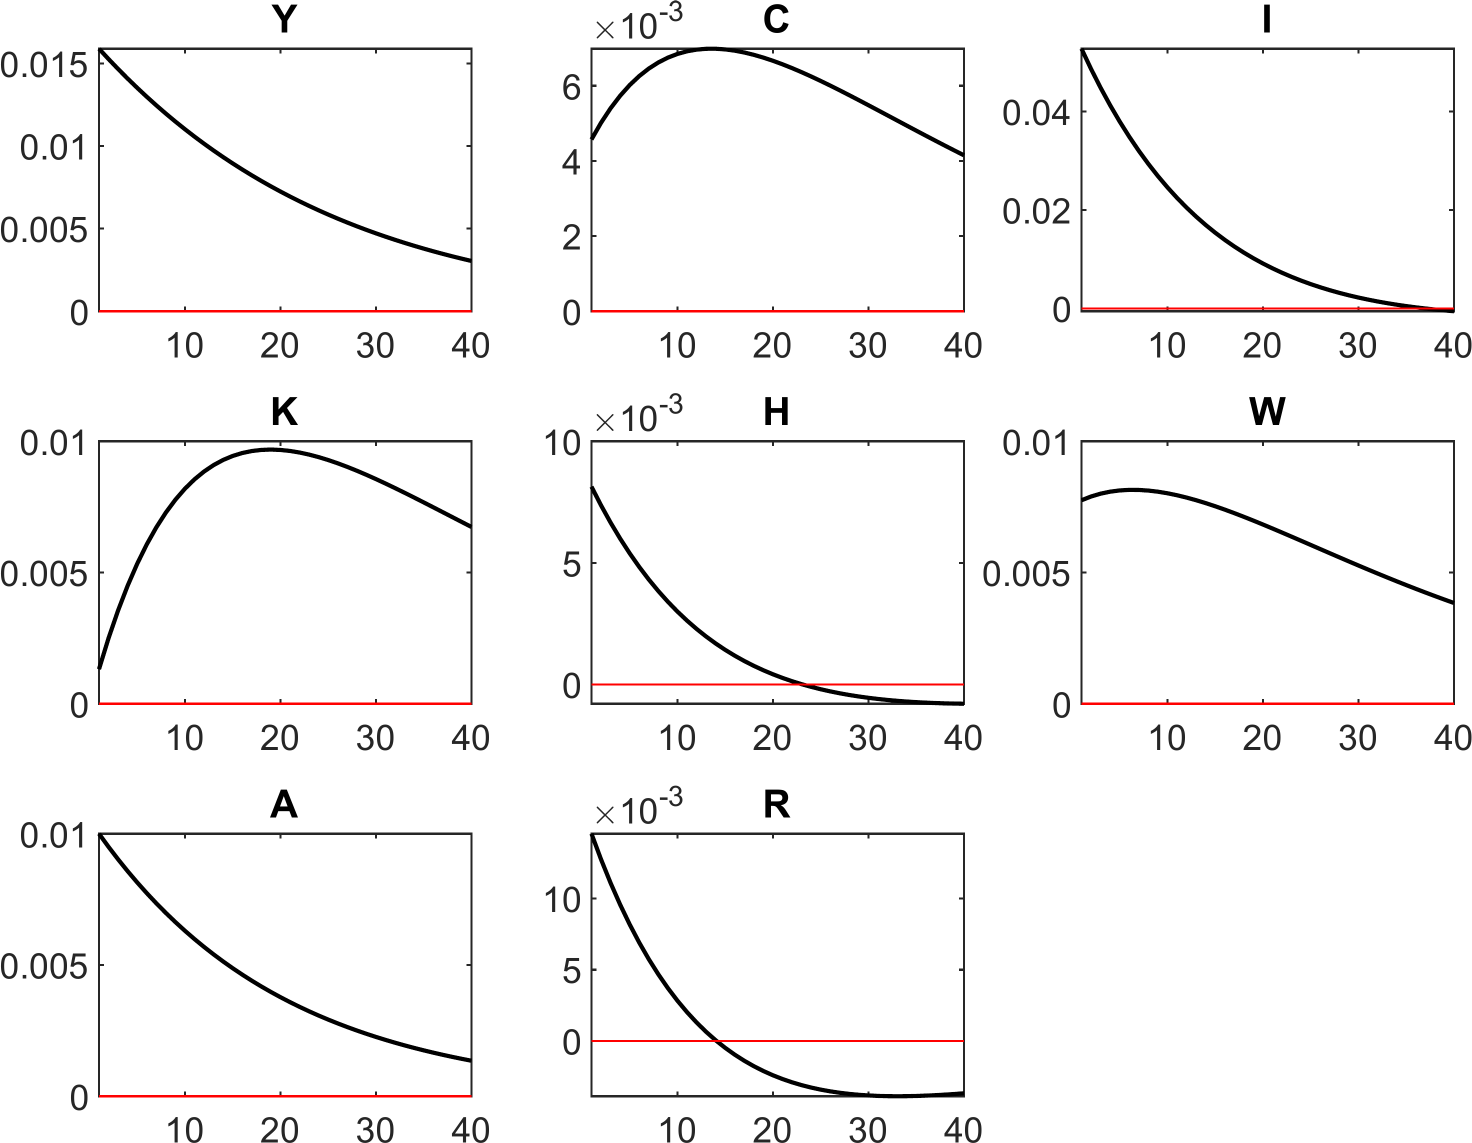
\includegraphics{code/rbc_model/rbc_model/graphs/rbc_model_IRF_eps_cropped.png}
\caption{image}
\end{figure}

\newpage
\newpage

\section{Appendix}\label{appendix}

\subsection{Households}\label{households-1}

\begin{align*}
  & \text{Define Lagrangian} \\
  & \mathcal{L} = \mathbb{E}_0 \sum_{t=1}^{\infty} \beta^{t-1} \Bigl\{
    \underbrace{\frac{\bigl(\tfrac{C_t}{P_t}-\eta\tfrac{C_{t-1}}{P_{t-1}}\bigr)^{1-\theta}}{1-\theta}}_{\text{Consumption utility}}
    - \underbrace{\chi\frac{h_t^{1+\gamma}}{1+\gamma}}_{\text{Labor disutility}}
    + \underbrace{\psi\ln\bigl(\tfrac{M_t}{P_t}\bigr)}_{\text{Money utility}} \\
  & \quad\qquad
    + \underbrace{\lambda_t\bigl[R^B_{t-1}B_{t-1}+M_{t-1}+W_th_t+R^k_tK_{t-1}+\Pi_t-P_t\tau_t-C_t-I_t-B_t-M_t\bigr]}_{\text{Nominal flow constraint}}
    + \underbrace{\mu_t\bigl[(1-\delta)K_{t-1}+I_t-\tfrac{\phi}{2}(\tfrac{I_t}{K_{t-1}}-\delta)^2K_{t-1}-K_t\bigr]}_{\text{Capital accumulation}}
  \Bigr\}
\end{align*}

\subsubsection{\texorpdfstring{First Order Conditions
\label{household_FOC}}{First Order Conditions }}\label{first-order-conditions}

\textbf{FOC w.r.t. Consumption} : \begin{align*}
  & \frac{\partial \mathcal{L}}{\partial C_t} = 0 \\
  & \quad \bigl[(c_t-\eta c_{t-1})^{-\theta}/P_t - \lambda_t\bigr]
    - \beta\,\mathbb{E}_t\bigl[\eta\,(c_{t+1}-\eta c_t)^{-\theta}/P_t\bigr] = 0 \\[6pt]
  & \text{Combine terms over }1/P_t \\
  & \quad \frac{1}{P_t}\bigl[(c_t-\eta c_{t-1})^{-\theta} - \beta\eta\,\mathbb{E}_t[(c_{t+1}-\eta c_t)^{-\theta}]\bigr] - \lambda_t = 0 \\[6pt]
  & \text{Multiply by }P_t \\
  & \quad (c_t-\eta c_{t-1})^{-\theta} - \beta\eta\,\mathbb{E}_t[(c_{t+1}-\eta c_t)^{-\theta}] - \lambda_t P_t = 0
\end{align*}

\begin{equation}\label{foc_C}
\boxed{
  \lambda_t P_t = (c_t-\eta c_{t-1})^{-\theta} - \beta\eta\,\mathbb{E}_t\bigl[(c_{t+1}-\eta c_t)^{-\theta}\bigr]
}
\end{equation}

\textbf{FOC w.r.t. Labour} : \begin{align*}
  & \frac{\partial \mathcal{L}}{\partial h_t} = 0 \\
  & \quad -\chi h_t^{\gamma} + \lambda_t W_t = 0 \\[6pt]
  & \text{Rearrange} \\
  & \quad \lambda_t W_t = \chi h_t^{\gamma}
\end{align*}

\begin{equation}\label{foc_h}
\boxed{\lambda_t W_t = \chi h_t^{\gamma}}
\end{equation}

\textbf{FOC w.r.t. Real Money Balances}: \begin{align*}
  & \frac{\partial \mathcal{L}}{\partial M_t} = 0 \\
  & \quad \beta^{t-1}\bigl[\psi/M_t - \lambda_t\bigr] + \beta^t\mathbb{E}_t[\lambda_{t+1}] = 0 \\[6pt]
  & \text{Divide by }\beta^{t-1}\text{ and rearrange} \\
  & \quad \psi/M_t - \lambda_t + \beta\,\mathbb{E}_t[\lambda_{t+1}] = 0
\end{align*}

\begin{equation}\label{foc_M}
\boxed{\frac{\psi}{M_t} = \lambda_t - \beta\,\mathbb{E}_t[\lambda_{t+1}]}
\end{equation}

\textbf{FOC w.r.t. Bonds} \eqref{foc_B}): \begin{align*}
  & \frac{\partial \mathcal{L}}{\partial B_t} = 0 \\
  & \quad -\beta^{t-1}\lambda_t + \beta^t\mathbb{E}_t[\lambda_{t+1}R^B_t] = 0 \\[6pt]
  & \text{Divide by }\beta^{t-1}\text{ and simplify} \\
  & \quad -\lambda_t + \beta\,\mathbb{E}_t[\lambda_{t+1}R^B_t] = 0
\end{align*}

\begin{equation}\label{foc_B}
\boxed{\lambda_t = \beta\,\mathbb{E}_t[\lambda_{t+1}R^B_t]}
\end{equation}

\textbf{FOC w.r.t. Capital} : \begin{align*}
  & \frac{\partial \mathcal{L}}{\partial K_t} = 0 \\
  & \quad -\beta^{t-1}\mu_t + \beta^t\mathbb{E}_t\bigl[\lambda_{t+1}R^k_{t+1} + \mu_{t+1}(1-\delta + \tfrac{\phi}{2}((I_{t+1}/K_t)^2 - \delta^2))\bigr] = 0 \\[6pt]
  & \text{Divide by }\beta^{t-1}\text{ and solve} \\
  & \quad \mu_t = \beta\,\mathbb{E}_t\bigl[\lambda_{t+1}R^k_{t+1} + \mu_{t+1}(1-\delta + \tfrac{\phi}{2}((I_{t+1}/K_t)^2 - \delta^2))\bigr]
\end{align*}

\begin{equation}\label{foc_K}
\boxed{\mu_t = \beta\,\mathbb{E}_t\bigl[\lambda_{t+1}R^k_{t+1} + \mu_{t+1}(1-\delta + \tfrac{\phi}{2}((I_{t+1}/K_t)^2 - \delta^2))\bigr]}
\end{equation}

\textbf{FOC w.r.t. Investment} : \begin{align*}
  & \frac{\partial \mathcal{L}}{\partial I_t} = 0 \\
  & \quad \beta^{t-1}\bigl[-\lambda_t + \mu_t(1 - \phi(\tfrac{I_t}{K_{t-1}} - \delta))\bigr] = 0 \\[6pt]
  & \text{Divide by }\beta^{t-1}\text{ and isolate} \\
  & \quad \lambda_t = \mu_t\bigl(1 - \phi(\tfrac{I_t}{K_{t-1}} - \delta)\bigr)
\end{align*}

\begin{equation}\label{foc_I}
\boxed{\lambda_t = \mu_t\bigl(1 - \phi(\tfrac{I_t}{K_{t-1}} - \delta)\bigr)}
\end{equation}

\subsubsection{Household Final
Equations}\label{household-final-equations}

\textbf{Consumption Euler Equation}\\
Combines consumption--habit dynamics with bond returns (from
\eqref{foc_B} and \eqref{foc_C}) :

\begin{align*}
& \text{Start with FOC for Bonds} \\
& \lambda_t = \beta\,\mathbb{E}_t[\lambda_{t+1}R_t^B] \quad \text{(Equation \ref{foc_B})} \\
& \\
& \text{Substitute } \lambda_t \text{ and } \lambda_{t+1} \text{ from FOC for Consumption} \\
& \lambda_t = \frac{(c_t - \eta\,c_{t-1})^{-\theta}}{P_t} \quad \text{(from Equation \ref{foc_C} rearranged)} \\
& \lambda_{t+1} = \frac{(c_{t+1} - \eta\,c_t)^{-\theta}}{P_{t+1}} \quad \text{(time-shifted)} \\
& \\
& \text{Combine results} \\
& \frac{(c_t - \eta\,c_{t-1})^{-\theta}}{P_t} = \beta\,\mathbb{E}_t\!\left[ R_t^B \cdot \frac{(c_{t+1} - \eta\,c_t)^{-\theta}}{P_{t+1}} \right] \\
& \\
& \text{Clear denominator} \\
& (c_t - \eta\,c_{t-1})^{-\theta} = \beta\,\mathbb{E}_t\!\left[ R_t^B \cdot \frac{P_t}{P_{t+1}} \cdot (c_{t+1} - \eta\,c_t)^{-\theta} \right]
\end{align*}

\begin{equation}\label{consEuler_app}
\boxed{%
  (c_t - \eta\,c_{t-1})^{-\theta}
  \;=\;
  \beta\,\mathbb{E}_t\!\Bigl[
    R_t^B \;\frac{P_t}{P_{t+1}}\;(c_{t+1} - \eta\,c_t)^{-\theta}
  \Bigr]
}
\end{equation}

\textbf{Labour Supply}

Real wage equals the marginal rate of substitution between leisure and
consumption (from \eqref{foc_C} and \eqref{foc_h}) :

\begin{align*}
& \text{Start with FOC for Hours Worked} \\
& \lambda_t W_t = \chi\,h_t^{\gamma} \quad \text{(Equation \ref{foc_h})} \\
& \\
& \text{Solve for } \lambda_t \\
& \lambda_t = \frac{\chi\,h_t^{\gamma}}{W_t} \\
& \\
& \text{Equate to FOC of Consumption expression} \\
& \frac{\chi\,h_t^{\gamma}}{W_t} = \frac{(c_t - \eta\,c_{t-1})^{-\theta} - \beta\,\eta\,\mathbb{E}_t[(c_{t+1} - \eta\,c_t)^{-\theta}]}{P_t} \\
& \\
& \text{Solve for real wage } (W_t/P_t) \\
& \frac{W_t}{P_t} = \frac{\chi\,h_t^{\gamma}}{(c_t - \eta\,c_{t-1})^{-\theta} - \beta\,\eta\,\mathbb{E}_t[(c_{t+1} - \eta\,c_t)^{-\theta}]}
\end{align*}

\begin{equation}\label{labourSupply_app}
\boxed{
  \frac{W_t}{P_t}
  \;=\;
  \frac{\chi\,h_t^{\gamma}}
       {(c_t - \eta\,c_{t-1})^{-\theta}
        \;-\;
        \beta\,\eta\,\mathbb{E}_t\!\bigl[(c_{t+1} - \eta\,c_t)^{-\theta}\bigr]}
}
\end{equation}

\textbf{Money Demand}\\
Opportunity cost of holding money vs.~bonds (from \eqref{foc_M},
\eqref{foc_B} and \eqref{foc_C}) :

\begin{align*}
& \text{Combine FOC for Money and Bonds} \\
& \frac{\psi}{M_t} = \lambda_t - \beta\,\mathbb{E}_t[\lambda_{t+1}] \quad \text{(Equation \ref{foc_M})} \\
& \lambda_t = \beta\,\mathbb{E}_t[\lambda_{t+1}R_t^B] \quad \text{(Equation \ref{foc_B})} \\
& \\
& \text{Substitute } \lambda_t \text{ into FOC of money} \\
& \frac{\psi}{M_t} = \beta\,\mathbb{E}_t[\lambda_{t+1}R_t^B] - \beta\,\mathbb{E}_t[\lambda_{t+1}] \\
& \frac{\psi}{M_t} = \beta\,\mathbb{E}_t\left[\lambda_{t+1}(R_t^B - 1)\right] \\
& \\
& \text{Substitute } \lambda_{t+1} \text{ from FOC of Consumption} \\
& \lambda_{t+1} = \frac{(c_{t+1} - \eta\,c_t)^{-\theta} - \beta\,\eta\,\mathbb{E}_{t+1}[(c_{t+2} - \eta\,c_{t+1})^{-\theta}]}{P_{t+1}} \\
& \\
& \text{Solve for } M_t \\
& M_t = \frac{\psi}{\beta\,\mathbb{E}_t\!\left[ (R_t^B - 1) \cdot \dfrac{(c_{t+1} - \eta\,c_t)^{-\theta} - \beta\,\eta\,\mathbb{E}_{t+1}[(c_{t+2} - \eta\,c_{t+1})^{-\theta}]}{P_{t+1}} \right]}
\end{align*}

\begin{equation}\label{money_demand_app}
\boxed{
  M_t
  \;=\;
  \frac{\psi}
       {\beta\,\mathbb{E}_t\!\Bigl[
         (R_t^B - 1)
         \;\cdot\;
         \dfrac{(c_{t+1} - \eta\,c_t)^{-\theta}
               \;-\;
               \beta\,\eta\,\mathbb{E}_{t+1}[(c_{t+2} - \eta\,c_{t+1})^{-\theta}]}
              {P_{t+1}}
       \Bigr]}
}
\end{equation}

\textbf{Capital Euler Equation } Defines Tobin's \(q\) and links
required returns on capital to bond returns (from \eqref{foc_I},
\eqref{foc_K} and \eqref{foc_B}) :

\begin{align*}
& \text{Define Tobin's } q \text{ from FOC for Investment} \\
& \lambda_t = \mu_t q_t \quad \text{where} \quad q_t \equiv 1 - \phi\left(\tfrac{I_t}{K_{t-1}} - \delta\right) \\
& \\
& \text{Rearrange FOC for Capital} \\
& \mu_t = \beta\,\mathbb{E}_t\!\left[ \lambda_{t+1}R_{t+1}^k + \mu_{t+1}\!\left(1-\delta + \tfrac{\phi}{2}\left[(I_{t+1}/K_t)^2 - \delta^2\right]\right) \right] \\
& \\
& \text{Substitute } \mu_t = \lambda_t / q_t \text{ and } \mu_{t+1} = \lambda_{t+1} / q_{t+1} \\
& \frac{\lambda_t}{q_t} = \beta\,\mathbb{E}_t\!\left[ \lambda_{t+1}R_{t+1}^k + \frac{\lambda_{t+1}}{q_{t+1}}\left(1-\delta + \tfrac{\phi}{2}\left[(I_{t+1}/K_t)^2 - \delta^2\right]\right) \right] \\
& \\
& \text{Factor } \lambda_{t+1} \\
& \frac{\lambda_t}{q_t} = \beta\,\mathbb{E}_t\!\left[ \lambda_{t+1} \left( R_{t+1}^k + \frac{1}{q_{t+1}}\left(1-\delta + \tfrac{\phi}{2}\left[(I_{t+1}/K_t)^2 - \delta^2\right]\right) \right) \right] \\
& \\
& \text{Substitute FOC for Bonds } (\lambda_t = \beta\,\mathbb{E}_t[\lambda_{t+1}R_t^B]) \\
& \frac{\beta\,\mathbb{E}_t[\lambda_{t+1}R_t^B]}{q_t} = \beta\,\mathbb{E}_t\!\left[ \lambda_{t+1} \left( R_{t+1}^k + \frac{1}{q_{t+1}}\Gamma_{t+1} \right) \right] \\
& \text{where } \Gamma_{t+1} \equiv 1-\delta + \tfrac{\phi}{2}\left[(I_{t+1}/K_t)^2 - \delta^2\right]
\end{align*}

\begin{equation}\label{capital_euler_app}
\boxed{
  \begin{gathered}
  q_t \;\equiv\; 1 - \phi\,\Bigl(\tfrac{I_t}{K_{t-1}} - \delta\Bigr) \\
  \\
  \frac{\beta\,\mathbb{E}_t\!\bigl[\lambda_{t+1}\,R_t^B\bigr]}{q_t}
  \;=\;
  \beta\,\mathbb{E}_t\!\Bigl[
    \lambda_{t+1}\Bigl(
      R_{t+1}^k
      + \frac{1}{q_{t+1}}
        \Bigl(
          1 - \delta
          + \tfrac{\phi}{2}\bigl[(I_{t+1}/K_t)^2 - \delta^2\bigr]
        \Bigr)
    \Bigr)
  \Bigr]
  \end{gathered}
}
\end{equation}

\subsection{Production}\label{production-1}

\subsubsection{\texorpdfstring{Final Good Producer
\label{final_good_producer_appendix}}{Final Good Producer }}\label{final-good-producer}

\textbf{Derivation of Intermediate Goods Demand and Aggregate Price
Index}

\begin{align*}  
& \text{Final goods producer's profit:} \\  
& \Pi_t = P_t Y_t - \int_0^1 P_t(j) Y_t(j)  dj \\  
& \text{subject to } Y_t = \left( \int_0^1 Y_t(j)^{\frac{\epsilon-1}{\epsilon}}  dj \right)^{\frac{\epsilon}{\epsilon-1}} \\  
& \\  
& \text{Substitute production function into profit:} \\  
& \Pi_t = P_t \left( \int_0^1 Y_t(j)^{\frac{\epsilon-1}{\epsilon}}  dj \right)^{\frac{\epsilon}{\epsilon-1}} - \int_0^1 P_t(j) Y_t(j)  dj \\  
& \\  
& \text{First-order condition for } Y_t(j): \\  
& \frac{\partial \Pi_t}{\partial Y_t(j)} = P_t \cdot \frac{\epsilon}{\epsilon-1} \left( \int_0^1 Y_t(i)^{\frac{\epsilon-1}{\epsilon}}  di \right)^{\frac{1}{\epsilon-1}} \cdot \frac{\epsilon-1}{\epsilon} Y_t(j)^{-\frac{1}{\epsilon}} - P_t(j) = 0 \\  
& \Rightarrow P_t \cdot Y_t^{\frac{1}{\epsilon}} Y_t(j)^{-\frac{1}{\epsilon}} = P_t(j) \\  
& \\  
& \text{Rearrange to obtain demand curve:} \\  
& Y_t(j) = \left( \frac{P_t}{P_t(j)} \right)^{\epsilon} Y_t \\  
& \\  
& \text{Substitute demand into production function:} \\  
& Y_t = \left( \int_0^1 \left[ \left( \frac{P_t}{P_t(j)} \right)^{\epsilon} Y_t \right]^{\frac{\epsilon-1}{\epsilon}}  dj \right)^{\frac{\epsilon}{\epsilon-1}} \\  
& = Y_t \left( \int_0^1 \left( \frac{P_t}{P_t(j)} \right)^{\epsilon-1}  dj \right)^{\frac{\epsilon}{\epsilon-1}} \\  
& \\
\end{align*} \begin{align*} 
& \text{Simplify to obtain price index:} \\  
& 1 = \left( \int_0^1 \left( \frac{P_t}{P_t(j)} \right)^{\epsilon-1}  dj \right)^{\frac{\epsilon}{\epsilon-1}} \\  
& \Rightarrow P_t^{1-\epsilon} = \int_0^1 P_t(j)^{1-\epsilon}  dj \\  
& \Rightarrow P_t = \left( \int_0^1 P_t(j)^{1-\epsilon}  dj \right)^{\frac{1}{1-\epsilon}}  
\end{align*}

\begin{equation}\label{demand_and_price}  
\boxed{  
  \begin{gathered}  
  Y_t(j) = \left( \frac{P_t(j)}{P_t} \right)^{-\epsilon} Y_t \\  
  \\  
  P_t = \left( \int_0^1 P_t(j)^{1-\epsilon}  dj \right)^{\frac{1}{1-\epsilon}}  
  \end{gathered}  
}  
\end{equation}

\subsubsection{\texorpdfstring{Intermediate Goods Producers
\label{intermediate_good_producer_appendix}}{Intermediate Goods Producers }}\label{intermediate-goods-producers-1}

\begin{align*}
& \text{Cost minimization for intermediate firm } j: \\
& \min_{K_t(j), h_t(j)} \left\{ R_t^k K_t(j) + W_t h_t(j) \right\} \\
& \text{subject to } Y_t(j) = A_t K_t(j)^{\alpha} h_t(j)^{1-\alpha} \\
& \\
& \text{Lagrangian:} \\
& \mathcal{L} = R_t^k K_t(j) + W_t h_t(j) + \lambda_t \left[ A_t K_t(j)^{\alpha} h_t(j)^{1-\alpha} - Y_t(j) \right] \\
& \\
& \text{First-order conditions:} \\
& \frac{\partial \mathcal{L}}{\partial K_t(j)} = 0: \quad R_t^k = \lambda_t \alpha A_t K_t(j)^{\alpha-1} h_t(j)^{1-\alpha} \\
& \frac{\partial \mathcal{L}}{\partial h_t(j)} = 0: \quad W_t = \lambda_t (1-\alpha) A_t K_t(j)^{\alpha} h_t(j)^{-\alpha} \\
& \\
& \text{Rearrange FOCs:} \\
& \lambda_t = \frac{R_t^k}{\alpha} \left( \frac{K_t(j)}{h_t(j)} \right)^{1-\alpha} \frac{1}{A_t}, \quad 
\lambda_t = \frac{W_t}{1-\alpha} \left( \frac{K_t(j)}{h_t(j)} \right)^{\alpha} \frac{1}{A_t} \\
& \\
& \text{Equate expressions:} \\
& \frac{R_t^k}{\alpha} \left( \frac{K_t(j)}{h_t(j)} \right)^{-\alpha} = \frac{W_t}{1-\alpha} \left( \frac{K_t(j)}{h_t(j)} \right)^{1-\alpha} \\
& \Rightarrow \frac{K_t(j)}{h_t(j)} = \frac{\alpha}{1-\alpha} \frac{W_t}{R_t^k} \\
& \\
& \text{Substitute into capital FOC:} \\
& \lambda_t = \frac{R_t^k}{\alpha A_t} \left( \frac{\alpha}{1-\alpha} \frac{W_t}{R_t^k} \right)^{\alpha-1} \\
& = \frac{1}{A_t} \left( \frac{R_t^k}{\alpha} \right)^{\alpha} \left( \frac{W_t}{1-\alpha} \right)^{1-\alpha}
\end{align*}

\begin{equation}\label{marginal_cost}
\boxed{MC_t = \dfrac{1}{A_t} \left( \dfrac{R_t^k}{\alpha} \right)^{\alpha} \left( \dfrac{W_t}{1-\alpha} \right)^{1-\alpha}}
\end{equation}

\begin{align*}
& \text{Intermediate‐goods producer’s problem:} \\
& \max_{P_t(j)} \;\mathbb{E}_t \sum_{s=0}^{\infty} \Lambda_{t,t+s}
  \Bigl[
    \bigl(\tfrac{P_{t+s}(j)}{P_{t+s}}\bigr)^{1-\epsilon} Y_{t+s}
    - mc_{t+s}\,\bigl(\tfrac{P_{t+s}(j)}{P_{t+s}}\bigr)^{-\epsilon} Y_{t+s}
    - \tfrac{\psi}{2}\bigl(\tfrac{P_{t+s}(j)}{P_{t+s-1}(j)} - 1\bigr)^2 Y_{t+s}
  \Bigr] \\
& \text{subject to} \quad Y_t(j) = \bigl(\tfrac{P_t(j)}{P_t}\bigr)^{-\epsilon} Y_t
\\[1.5ex]
& \text{First‐Order Condition w.r.t. }P_t(j): \\
& \mathbb{E}_t\Bigl[
    \frac{\partial \Pi_t(j)}{\partial P_t(j)}
    + \beta\,\Lambda_{t,t+1}
      \frac{\partial \Pi_{t+1}(j)}{\partial P_t(j)}
  \Bigr] = 0
\\[1ex]
& \frac{\partial \Pi_t}{\partial P_t(j)}
  = (1-\epsilon)\bigl(\tfrac{P_t(j)}{P_t}\bigr)^{-\epsilon}\tfrac{Y_t}{P_t}
    + \epsilon\,mc_t\bigl(\tfrac{P_t(j)}{P_t}\bigr)^{-\epsilon-1}\tfrac{Y_t}{P_t}
    - \psi\bigl(\tfrac{P_t(j)}{P_{t-1}(j)}-1\bigr)\tfrac{Y_t}{P_{t-1}(j)}
\\[1ex]
& \frac{\partial \Pi_{t+1}}{\partial P_t(j)}
  = \psi\bigl(\tfrac{P_{t+1}(j)}{P_t(j)}-1\bigr)\,\tfrac{P_{t+1}(j)}{P_t(j)^2}\,Y_{t+1}
\\[2ex]
& \text{Impose symmetry: }P_t(j)=P_t,\;Y_t(j)=Y_t,\;\pi_t=\tfrac{P_t}{P_{t-1}}.\\
& (1-\epsilon)+\epsilon\,mc_t = \epsilon\bigl(mc_t-\tfrac{\epsilon-1}{\epsilon}\bigr),\quad
  \tfrac{P_t(j)}{P_{t-1}(j)}=\pi_t,\;\tfrac{P_{t+1}(j)}{P_t(j)}=\pi_{t+1}
\\[1ex]
& 0 = \epsilon\bigl(mc_t-\tfrac{\epsilon-1}{\epsilon}\bigr)
      - \psi\,(\pi_t-1)\,\pi_t
      + \beta\,\mathbb{E}_t\Bigl[
          \Lambda_{t,t+1}\,\psi\,(\pi_{t+1}-1)\,\pi_{t+1}
          \,\tfrac{Y_{t+1}P_t}{Y_tP_{t+1}}
        \Bigr]
\\[1ex]
\end{align*}

Noting \(\Lambda_{t,t+1}=\beta\,\tfrac{\lambda_{t+1}}{\lambda_t}\) and
\(P_{t+1}/P_t=\pi_{t+1}\), the bracket simplifies to
\(\beta\,\tfrac{\lambda_{t+1}}{\lambda_t}\,\tfrac{Y_{t+1}}{Y_t}\).

\begin{equation}\label{rotemberg_FOC}
\boxed{
  0 = \epsilon\Bigl(mc_t - \tfrac{\epsilon-1}{\epsilon}\Bigr)
      - \psi\,(\pi_t - 1)\,\pi_t
      + \beta\,\mathbb{E}_t\!
        \Bigl[
          \tfrac{\lambda_{t+1}}{\lambda_t}\,
          \psi\,(\pi_{t+1}-1)\,\pi_{t+1}\,
          \tfrac{Y_{t+1}}{Y_t}
        \Bigr]
}
\end{equation}

\newpage

\newpage

\section{Old Stuff}\label{old-stuff}

Components breakdown:

Expenditures:

Consumption: \(P_t c_t\)

Investment: \(P_t i_t\)

Bonds: \(B_t\)

Money holdings: \(M_t\)

Income sources:

Bond returns: \((1 + i_{t-1}) B_{t-1}\)

Money carryover: \(M_{t-1}\)

Labor income: \(W_t h_t\)

Capital returns: \(R_t^k K_{t-1}\) (Key addition missing in Sims)

Firm profits: \(\Pi_t\)

Net transfers: \(-P_t \tau_t\)

\newpage

\section*{References}\label{references}
\addcontentsline{toc}{section}{References}

\phantomsection\label{refs}
\begin{CSLReferences}{1}{1}
\bibitem[\citeproctext]{ref-ecbwp770}
European Central Bank. 2022. \emph{Economic and monetary developments
no. 770}. (ECB Working Paper 770). European Central Bank. {[}Online{]},
Available: \url{https://www.ecb.europa.eu/pub/pdf/scpwps/ecbwp770.pdf}.

\bibitem[\citeproctext]{ref-Mati2019}
Mati, S. 2019. DynareR: Bringing the power of {Dynare} to {R}, {R
Markdown}, and {Quarto}. \emph{CRAN}. {[}Online{]}, Available:
\url{https://CRAN.R-project.org/package=DynareR}.

\bibitem[\citeproctext]{ref-sims2024newkeynesian}
Sims, E. 2024a. \emph{Graduate macro theory II: The basic new keynesian
model}. (Lecture Notes ECON 60202 -- Spring 2024). Notre Dame, IN:
University of Notre Dame. {[}Online{]}, Available:
\url{https://sites.nd.edu/esims/files/2024/03/notes_new_keynesian_2024-1.pdf}.

\bibitem[\citeproctext]{ref-sims2024rbc}
Sims, E. 2024b. \emph{Graduate macro theory II: Extensions of basic RBC
framework}. (Lecture Notes ECON 60202 -- Spring 2024). Notre Dame, IN:
University of Notre Dame. {[}Online{]}, Available:
\url{https://sites.nd.edu/esims/files/2024/02/notes_rbc_extensions_2024.pdf}.

\bibitem[\citeproctext]{ref-sims2024fiscal}
Sims, E. 2024c. \emph{Fiscal policy in the RBC model}. (Lecture Notes
ECON 60202 -- Spring 2024). Notre Dame, IN: University of Notre Dame.
{[}Online{]}, Available:
\url{https://sites.nd.edu/esims/files/2024/02/notes_fiscal_policy_2024.pdf}.

\end{CSLReferences}

\bibliography{Tex/ref}





\end{document}
